\documentclass[]{article}
\usepackage{lmodern}
\usepackage{amssymb,amsmath}
\usepackage{ifxetex,ifluatex}
\usepackage{fixltx2e} % provides \textsubscript
\ifnum 0\ifxetex 1\fi\ifluatex 1\fi=0 % if pdftex
  \usepackage[T1]{fontenc}
  \usepackage[utf8]{inputenc}
\else % if luatex or xelatex
  \ifxetex
    \usepackage{mathspec}
  \else
    \usepackage{fontspec}
  \fi
  \defaultfontfeatures{Ligatures=TeX,Scale=MatchLowercase}
\fi
% use upquote if available, for straight quotes in verbatim environments
\IfFileExists{upquote.sty}{\usepackage{upquote}}{}
% use microtype if available
\IfFileExists{microtype.sty}{%
\usepackage{microtype}
\UseMicrotypeSet[protrusion]{basicmath} % disable protrusion for tt fonts
}{}
\usepackage[margin=1in]{geometry}
\usepackage{hyperref}
\hypersetup{unicode=true,
            pdftitle={Assignment 3},
            pdfauthor={Sri Seshadri},
            pdfborder={0 0 0},
            breaklinks=true}
\urlstyle{same}  % don't use monospace font for urls
\usepackage{longtable,booktabs}
\usepackage{graphicx,grffile}
\makeatletter
\def\maxwidth{\ifdim\Gin@nat@width>\linewidth\linewidth\else\Gin@nat@width\fi}
\def\maxheight{\ifdim\Gin@nat@height>\textheight\textheight\else\Gin@nat@height\fi}
\makeatother
% Scale images if necessary, so that they will not overflow the page
% margins by default, and it is still possible to overwrite the defaults
% using explicit options in \includegraphics[width, height, ...]{}
\setkeys{Gin}{width=\maxwidth,height=\maxheight,keepaspectratio}
\IfFileExists{parskip.sty}{%
\usepackage{parskip}
}{% else
\setlength{\parindent}{0pt}
\setlength{\parskip}{6pt plus 2pt minus 1pt}
}
\setlength{\emergencystretch}{3em}  % prevent overfull lines
\providecommand{\tightlist}{%
  \setlength{\itemsep}{0pt}\setlength{\parskip}{0pt}}
\setcounter{secnumdepth}{0}
% Redefines (sub)paragraphs to behave more like sections
\ifx\paragraph\undefined\else
\let\oldparagraph\paragraph
\renewcommand{\paragraph}[1]{\oldparagraph{#1}\mbox{}}
\fi
\ifx\subparagraph\undefined\else
\let\oldsubparagraph\subparagraph
\renewcommand{\subparagraph}[1]{\oldsubparagraph{#1}\mbox{}}
\fi

%%% Use protect on footnotes to avoid problems with footnotes in titles
\let\rmarkdownfootnote\footnote%
\def\footnote{\protect\rmarkdownfootnote}

%%% Change title format to be more compact
\usepackage{titling}

% Create subtitle command for use in maketitle
\newcommand{\subtitle}[1]{
  \posttitle{
    \begin{center}\large#1\end{center}
    }
}

\setlength{\droptitle}{-2em}
  \title{Assignment 3}
  \pretitle{\vspace{\droptitle}\centering\huge}
  \posttitle{\par}
  \author{Sri Seshadri}
  \preauthor{\centering\large\emph}
  \postauthor{\par}
  \predate{\centering\large\emph}
  \postdate{\par}
  \date{8/5/2018}

\usepackage{float}

\begin{document}
\maketitle

\section{Problem 1}\label{problem-1}

Here there are two scenarios that will be inspected using Integer Linear
Programming (ILP) to model total cost. Scenario 1 - plant in Baltimore,
Scenario 2 - plant in Seattle.

\subsection{Executive Summary:}\label{executive-summary}

Both Scenarios yield a total cost of \$9,900, therefore any location
between Baltimore and Seattle can be chosen.

\subsection{Scenario 1}\label{scenario-1}

\subsubsection{Formulation:}\label{formulation}

The model is formulated as a network flow model as shown in the figure
below, where nodes 1 through 5 are Los Angeles, Baltimore, Atlanta,
Tulsa and New York respectively

\begin{center}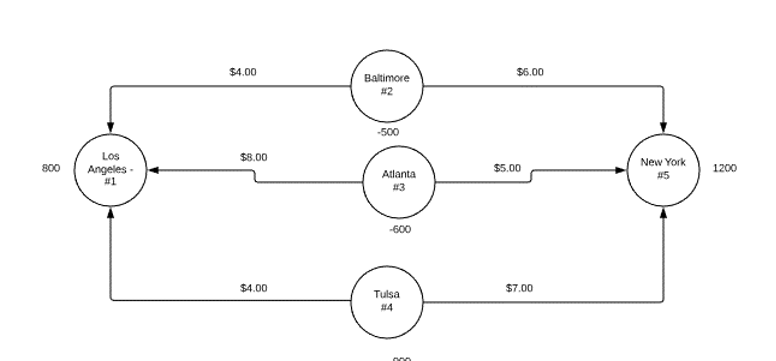
\includegraphics[width=10.78in]{Figures/Homework3/1aFig} \end{center}

\paragraph{Decision variables:}\label{decision-variables}

Let \(X_{ij}\) be the flow from node \(i\) to \(j\) where
\(i\in \{2,3,4\}\) and \(j \in \{1,5\}\)

\(X_{ij}\) are the decision variables.

\paragraph{Other variables}\label{other-variables}

Let \(C_{ij}\) be the cost variable for distribution of toys between
\(X_ij\) Let \(D_{i}\) be the supply at \(i\) and \(D_{j}\) be the
demand at \(j\). \(D_{i}\) is denoted with a negative number and the
\(D_{j}\) as positive number for modeling as a network flow problem.

\paragraph{Objective function}\label{objective-function}

\(Min\) \(Total Cost\) = \(X_{ij}C_{ij}\)

\paragraph{Constraints:}\label{constraints}

Since the supply equals the demand (\(\sum_{i}D_{i}\) \(+\)
\(\sum_{j}D_{j} = 0\)), the model will be constrained as
\(Inflow - Outflow = Supply\) \(or\) \(Demand\).

The constraints in explicit form are:

\(X_{21} + X_{31} + X_{41} - 0 = D_{1}\) where \(D_{1} = 800\)
\(X_{25} + X_{35} + X_{45} - 0 = D_{5}\) where \(D_{5} = 1200\)

\(0 - X_{21} - X_{25} = D_{2}\) Where \(D_{2} = -500\)
\(0 - X_{31} - X_{35} = D_{3}\) Where \(D_{3} = -600\)
\(0 - X_{41} - X_{45} = D_{4}\) Where \(D_{2} = -900\)

\(X_{ij} > = 0\) and \(X_{ij}\) are integers

\subsubsection{ASME Modeling}\label{asme-modeling}

Figures 1 and 2 show the model set up in ASPE

\begin{figure}[h]

{\centering 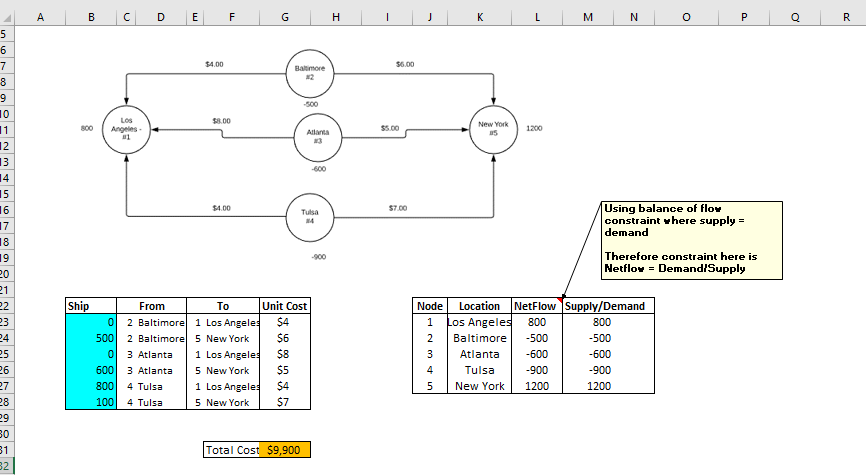
\includegraphics[width=12.03in]{Figures/Homework3/p1a} 

}

\caption{ASPE formulation - Baltimore scenario}\label{fig:unnamed-chunk-2}
\end{figure}

\begin{figure}[h]

{\centering 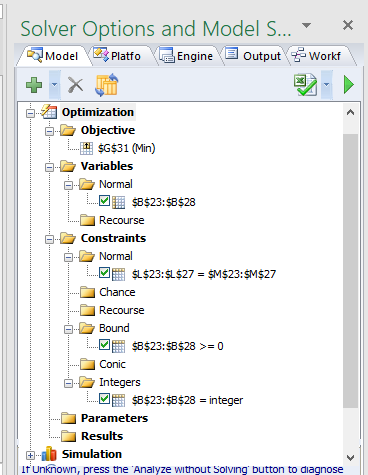
\includegraphics[width=5.11in]{Figures/Homework3/modelp1a} 

}

\caption{ASPE Model Setup - Baltimore scenario}\label{fig:unnamed-chunk-3}
\end{figure}

\subsubsection{Scenario 1 Results}\label{scenario-1-results}

The Total cost for a plant in Baltimore was \$9900

\pagebreak

\subsection{Scenario 2}\label{scenario-2}

This is scenario is identical to the previous scenario but the node 2 is
replaced with node 6 (seattle) and its respective costs for distribution
to Node 1 and 5. The formulation is not repeated here fro brevity. The
model set up is shown in figures 3 and 4

The Total cost for a plant in Seattle was \$9900. Therefore the either
of the scenarios would work for the Toy company.

\begin{figure}[h]

{\centering 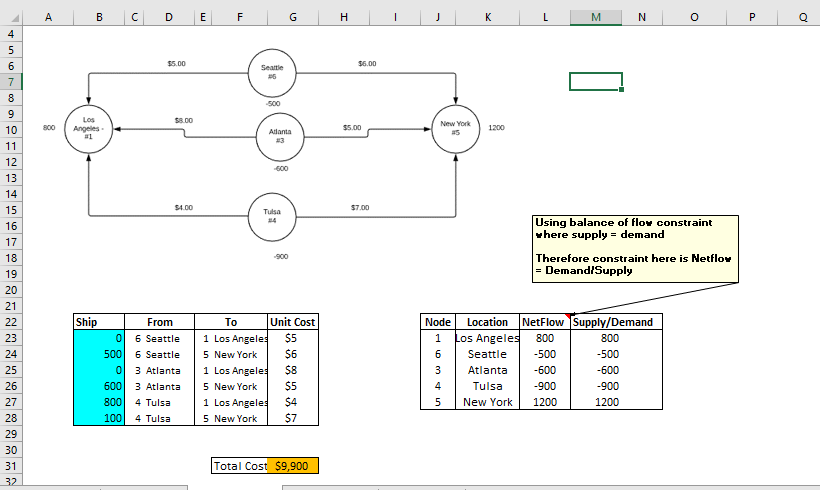
\includegraphics[width=11.39in]{Figures/Homework3/p1b} 

}

\caption{ASPE formulation - Seattle scenario}\label{fig:unnamed-chunk-4}
\end{figure}

\begin{figure}[h]

{\centering 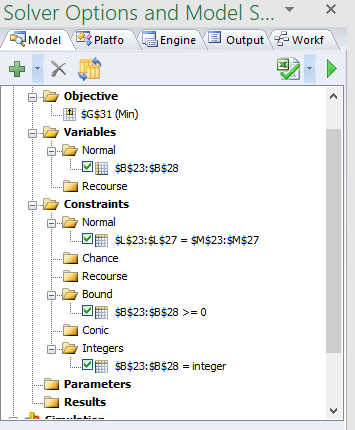
\includegraphics[width=4.93in]{Figures/Homework3/modelp1b} 

}

\caption{ASPE Model Setup - Seattle scenario}\label{fig:unnamed-chunk-5}
\end{figure}

\pagebreak

\section{Problem 2}\label{problem-2}

In this problem, the economical combination of four meats for hot dog is
formuated as a linear program. The units of weight measures are
standardized to grams and all figures are reported in grams except for
calories and cost.

\subsection{Executive Summary:}\label{executive-summary-1}

The economical combination would be 14.175 grams of beef and pork and
28.35 grams of turkey. The cost of 2 ounce hot dog would be \$0.086

\subsection{Formulation}\label{formulation-1}

\subsubsection{Decision variables}\label{decision-variables-1}

Let \(X_{i}\) be the amount of meat used for hot dog where
\(i \in \{Beef,Pork, Chicken, Turkey\}\).

\subsubsection{Other variables}\label{other-variables-1}

Let \(D_{i},K_{i},F_{i},L_{i}\) be the Cost, Calories, Fat(grams) and
Cholestrol(grams) per gram of hot dog respectively where
\(i \in \{Beef,Pork, Chicken, Turkey\}\).

\subsubsection{Objective function}\label{objective-function-1}

\(Min\) \(\sum_{i}X_{i}D_{i}\)

\subsubsection{Constraints}\label{constraints-1}

\(\sum_{i}X_{i} = 56.7\) (2 ounces = 56.7 grams)
\(X_{Chicken} + X_{Turkey} > 0\) (Use of either Chicken or Turkey or
both)

Note that in the ASPE, there is no greater than constraint and so
greater than on equal to a very small number (0.0000001) was used to
model.

\(\sum_{i}X_{i}F_{i} <= 6\) Total Fat constraint

\(\sum_{i}X_{i}L_{i} <= 27\) Total Cholestrol constraint

\(\sum_{i}X_{i}K_{i} <= 100\) Total Calories constraint

\(X_{ij} > = 0\)

\subsection{ASPE Modeling}\label{aspe-modeling}

Figures 5 shows the model set up

\begin{figure}
\centering
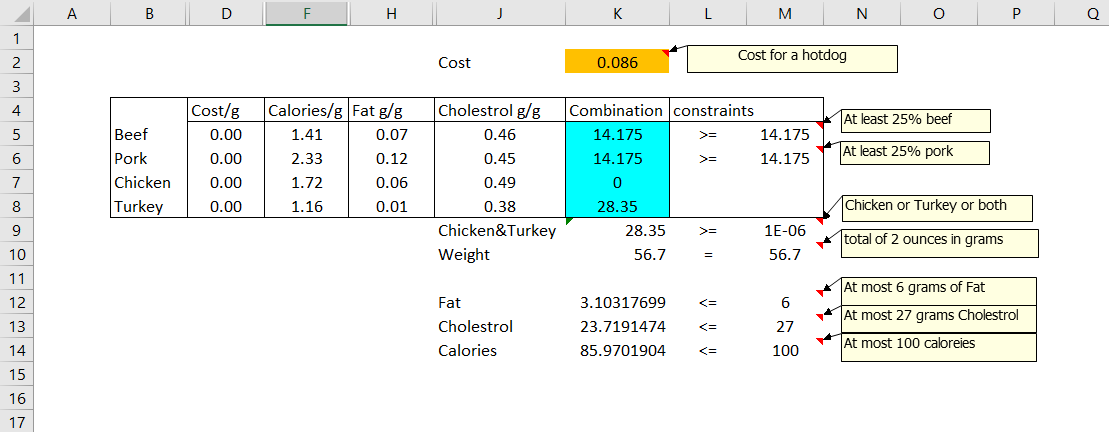
\includegraphics[height=0.50000\textwidth]{Figures/Homework3/p2.PNG}
\caption{Problem 2 ASPE formulation}
\end{figure}

\subsection{Result}\label{result}

The economical combination would be 14.175 grams of beef and pork and
28.35 grams of turkey. The cost of 2 ounce hot dog would be \$0.086

\section{Problem 3}\label{problem-3}

\subsection{Executive Summary}\label{executive-summary-2}

For 5 Surgery problem, the schedule is as shown in figure 6 with a total
setup time of 58. The cost is shown next to the arcs

\begin{figure}[h]

{\centering 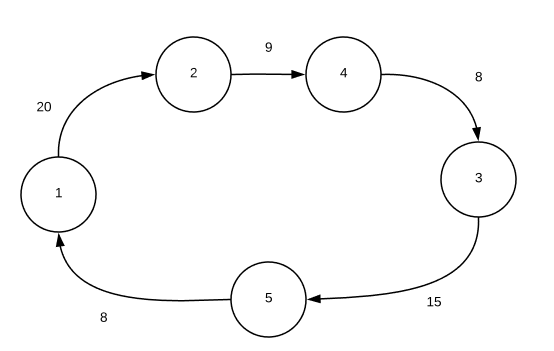
\includegraphics[width=7.69in]{Figures/Homework3/p3aS} 

}

\caption{5 surgery schedule}\label{fig:unnamed-chunk-6}
\end{figure}

For the 10 surgery problem, the schedule is shown in figure 7 with a
total setup time of 92.

\begin{figure}[h]

{\centering 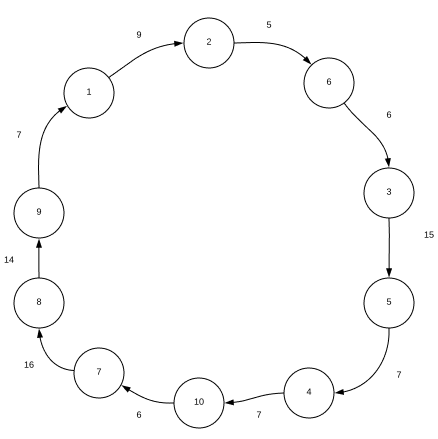
\includegraphics[width=6.08in]{Figures/Homework3/p3bS} 

}

\caption{10 surgery schedule}\label{fig:unnamed-chunk-7}
\end{figure}

\subsection{Formulation}\label{formulation-2}

The formulation is not reproduced here from the paper. However an
attempt was made to make the schedule continuous in ASPE by using a
dummy cost parameter.

\(dummyCost_{i=j} = 1000 - 1000* \sum_{i}X_{ij}\) \(\forall_{j} \in N\)

That is, if a schedule ends in node 2, \(\sum_{i}X_{i2} = 1\), then
\(dummyCost_{i=2} = 0\), which encourages the model to schedule a
surgery starting from 2. Else the cost would be 1000.

Also, We need to prevent schedules that re-traces a path example
1-\textgreater{}5 -\textgreater{} 1

\(X_{12} + X_{21} <= 1\) \(X_{13} + X_{31} <= 1\)
\(X_{14} + X_{41} <= 1\) \(X_{15} + X_{51} <= 1\)
\(X_{23} + X_{32} <= 1\)

So on \ldots{}

\subsection{ASPE Model set up for 5 surgery
problem}\label{aspe-model-set-up-for-5-surgery-problem}

Figures 8 and 9 show the ASPE model set up

\begin{figure}
\centering
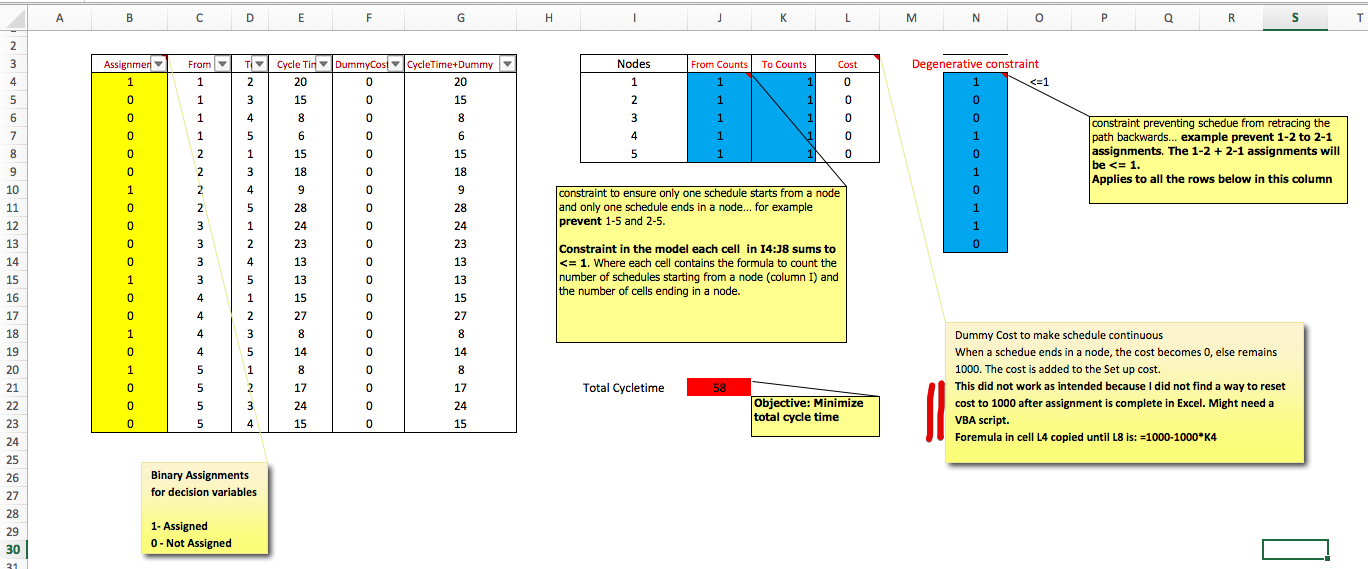
\includegraphics[height=0.50000\textwidth]{Figures/Homework3/p3a.PNG}
\caption{5 surgery ASPE formulation}
\end{figure}

\begin{figure}
\centering
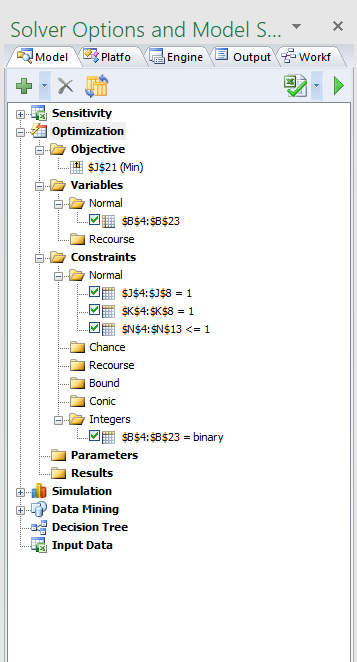
\includegraphics[height=0.50000\textwidth]{Figures/Homework3/modelp3a.PNG}
\caption{5 surgery ASPE model set up}
\end{figure}

\subsection{5 Surgery problem result}\label{surgery-problem-result}

The schedule is
1-\textgreater{}2-\textgreater{}4-\textgreater{}3-\textgreater{}5 With a
total setup time of 58

\subsection{ASPE Model set up for 10 surgery
problem}\label{aspe-model-set-up-for-10-surgery-problem}

The model set up identical to the 5 surgery problem (as shown in figure
11 and 12). For brevity the model is shown by filtering on
\(X_{ij} = 1\). The dummy cost did not help with keeping the schedule
continuous. There was a degenerative schedule as a result of this type
of model. the schedule is shown in figure 10.

\begin{figure}
\centering
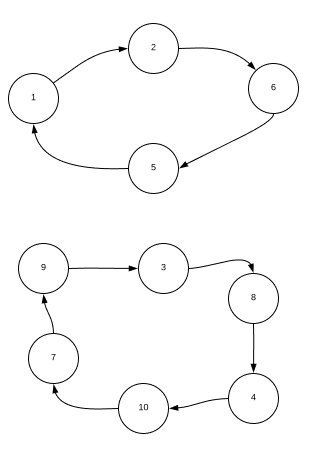
\includegraphics[height=0.50000\textwidth]{Figures/Homework3/p3bsnW.PNG}
\caption{10 surgery degenerative schedule}
\end{figure}

When \(X_{51} = 0\) constraint was added to the model, then a plausible
schedule resulted.

\begin{figure}
\centering
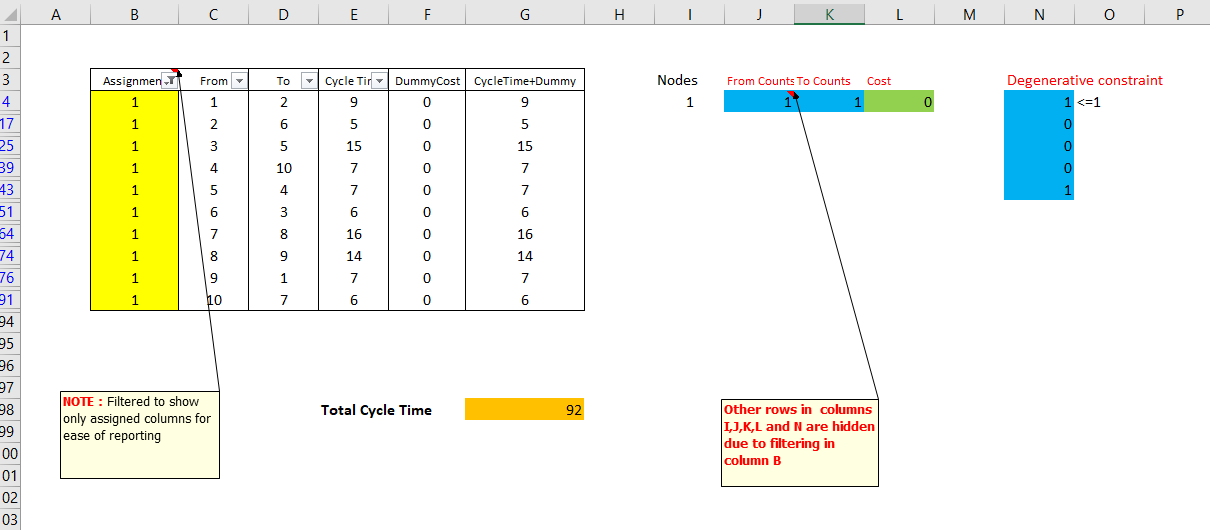
\includegraphics[height=0.50000\textwidth]{Figures/Homework3/p3b.PNG}
\caption{10 surgery ASPE formulation}
\end{figure}

\begin{figure}
\centering
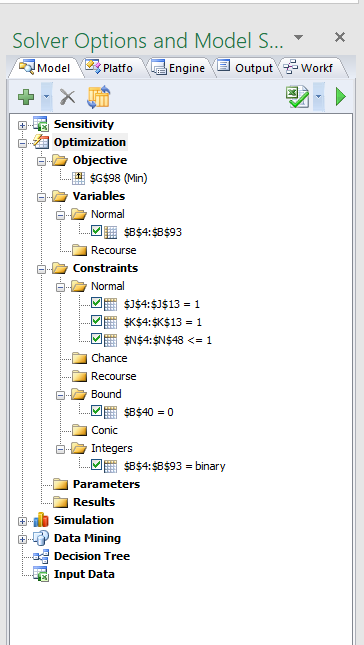
\includegraphics[height=0.50000\textwidth]{Figures/Homework3/modelp3b.PNG}
\caption{10 surgery ASPE model set up}
\end{figure}

\subsection{10 Surgery problem result}\label{surgery-problem-result-1}

As shown in figure 10, the schedule is

1-\textgreater{}2 -\textgreater{} 6 -\textgreater{} 3 -\textgreater{} 5
-\textgreater{} 4 -\textgreater{} 10 -\textgreater{} 7 -\textgreater{} 8
-\textgreater{} 9 -\textgreater{} 1, with a total setup time of 92.

\section{Problem 4}\label{problem-4}

\subsection{Data}\label{data}

\begin{longtable}[]{@{}lrrrr@{}}
\toprule
& Tank & Truck & Turtle & Available\tabularnewline
\midrule
\endhead
Plastic & 1.5 & 2.0 & 1 & 16000\tabularnewline
Rubber & 0.5 & 0.5 & 1 & 5000\tabularnewline
Metal & 0.3 & 0.6 & 0 & 9000\tabularnewline
Labor & 2.0 & 2.0 & 1 & 40\tabularnewline
Cost & 7.0 & 5.0 & 4 & 164000\tabularnewline
\bottomrule
\end{longtable}

\subsection{Goals}\label{goals}

\begin{itemize}
\tightlist
\item
  Minimize over-utilization of Plastic, Rubber and Metal with twice the
  emphasis on Plastic.
\item
  Minimize the under and over utilizations of the budget
\item
  Maximize labor utilization
\end{itemize}

\subsection{Decision Variables}\label{decision-variables-2}

Let \(X_{1}, X_{2}\) and \(X_{3}\) be the number of Tanks, Trucks and
Turtles made.

\subsection{Goal Constraint:}\label{goal-constraint}

\(1.5X_{1} + 2X_{2} + X_{3} - d_{p}^{+} + d_{p}^{-} = 16000\) (plastic
usage)

\(0.5X_{1} + 0.5X_{2} + X_{3} - d_{r}^{+} + d_{r}^{-} = 5000\) (rubber
usage)

\(0.3X_{1} + 0.6X_{2} - d_{m}^{+} + d_{m}^{-} = 9000\) (metal usage)

\(2X_{1} + 2X_{2} + X_{3} - d_{l}^{+} + d_{l}^{-} = 40\) (labor usage)

\(7X_{1} + 5X_{2} + 4X_{3} - d_{c}^{+} + d_{c}^{-} = 164000\) (budget
usage)

Where \(d_{p}^{+},d_{r}^{+},d_{m}^{+},d_{l}^{+},d_{c}^{+}\) are over
achieving deviational varibles and
\(d_{p}^{-},d_{r}^{-},d_{m}^{-},d_{l}^{-},d_{c}^{-}\) are under
achieving deviational varibles

\(d_{p}^{+},d_{r}^{+},d_{m}^{+},d_{l}^{+},d_{c}^{+},d_{p}^{-},d_{r}^{-},d_{m}^{-},d_{l}^{-},d_{c}^{-} >= 0\)
and integer \(X_{i} >= 0\) and integer

\subsection{Objective function}\label{objective-function-2}

\(Min\)
\(w_{r}\frac {(d_{p}^{+})}{5000} + w_{m} \frac {d_{m}^{+}}{9000} + w_{p} \frac {d_{p}^{+}}{16000} + w_{l}\frac{d_{l}^{-}}{40} + w_{c}\frac{d_{c}^{+}+d_{c}^{-}}{164000}\)

where the \(w_{r},w_{m},w_{l},w_{c} = 1\) and \(w_{p} = 2\)

\pagebreak

\section{Problem 5}\label{problem-5}

\subsection{Goals}\label{goals-1}

\begin{itemize}
\tightlist
\item
  Achieve total exposures of atleast 750,000 persons
\item
  Avoid expenditures of more than \$100,000
\item
  Avoid expenditures of \textgreater{} \$70,000 for TV advertisements
\item
  Achieve at least 1 Million total expenditures
\item
  Reach at least 250,000 persons in each of the two age groups 18-21 and
  25-30.
\item
  In addition purchasing power of 25-30 is twice as much of 18-21 group.
\end{itemize}

\subsection{Decision Variables}\label{decision-variables-3}

\(X_{1}\) be the dollar amount spent on TV campaign \textbf{in 1000s of
dollars}

\(X_{2}\) be the dollar amount spent on Radio campaign \textbf{in 1000s
of dollars}

\subsection{Goal constraints}\label{goal-constraints}

\(5500X_{1} + 4500X_{2} + d_{p}^{-} - d_{p}^{+} = 750000\) (goal 1)

\(X_{1} + X_{2} + d_{c}^{-} - d_{c}^{+} = 100\) (goal 2)

\(X_{1} + d_{t}^{-} - d_{t}^{+} = 70\) (goal 3)

\(10000X_{1} + 7500X_{2} + d_{e}^{-}-d_{e}^{+}= 1000000\) (goal 4)

\(2500X_{1} + 3000X_{2} + d_{18-21}^{-} + d_{18-21}^{+} = 250000\) (goal
5)

\(3000X_{1} + 1500X_{2} + d_{25-30}^{-} + d_{25-30}^{+} = 250000\) (goal
5)

\subsection{Objective function}\label{objective-function-3}

\(Min\)
\(w_{1} \frac{d_{p}^{-}}{750000} + w_{2} \frac{d_{c}^{+}}{100} + w_{3}\frac{d_{t}^{+}}{70} + w_{4}\frac{d_{e}^{-}}{1000000} + w_{5}\frac{0.5*d_{18-21}^{-} + d_{25-30}^{-}}{250000}\)

\(w_{1} = 5, w_{2} = 4, w_{3} = 3, w_{4} = 2, w_{1} = 1\)

Further there is a weight of 0.5 was given to \(d_{18-21}^{-}\) to
account for purchasing power of 18-21 group being half of 25-30.

\section{Extra Credit}\label{extra-credit}

\subsection{a) The different patterns that may be used
are}\label{a-the-different-patterns-that-may-be-used-are}

\begin{itemize}
\tightlist
\item
  2 5ft pieces cut
\item
  3 3ft pieces cut
\item
  2 4ft pieces cut
\item
  2 3ft pieces and 1 4ft piece cut
\item
  1 4ft piece and 1 5ft piece cut
\item
  1 3ft piece and 1 5ft piece cut
\end{itemize}

\subsection{b) Formulation}\label{b-formulation}

\subsubsection{Decision Variables:}\label{decision-variables-4}

Let \(X_{i}\) be the number of boards used to cut in the pattern \(i\),
where \(i\) belongs to the patterns described in the same order as
above.

\subsubsection{Objective}\label{objective}

\(Min\) \(\sum_{i} X_{i}\)

\subsubsection{Constraints}\label{constraints-2}

\(3X_{2} + 2X_{4} + x_{6} >= 90\) (number of 3 feet board requirement)

\(2X_{3} + X_{4} + X_{5} >= 60\) (number of 4 feet board requirement)

\(2X_{1} + X_{5} + X_{6} >= 60\) (number of 5 feet board requirement)

\(X_{i} > 0\) and \(integers\)

\subsubsection{ASME Formulation}\label{asme-formulation}

Shown in figure 13 and 14

\begin{figure}
\centering
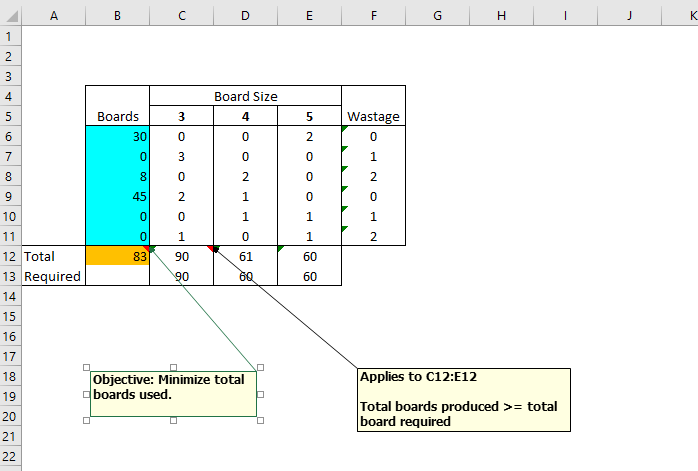
\includegraphics[height=0.50000\textwidth]{Figures/Homework3/pEC.PNG}
\caption{Lumberyard ASPE Model setup}
\end{figure}

\begin{figure}
\centering
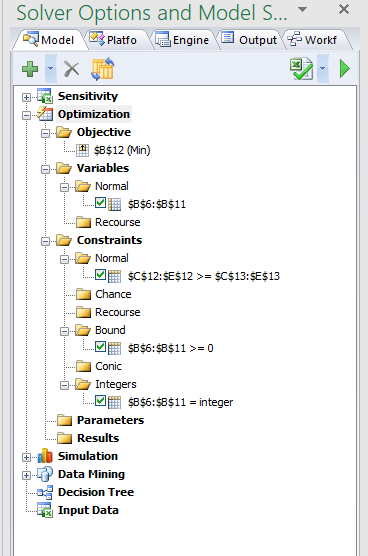
\includegraphics[height=0.40000\textwidth]{Figures/Homework3/modelpEC.PNG}
\caption{Lumberyard ASPE Model constraints}
\end{figure}

\pagebreak

\subsubsection{Result}\label{result-1}

\begin{itemize}
\tightlist
\item
  \emph{30 boards} for 2 5ft pieces cut
\item
  \emph{None} for 3 3ft pieces cut
\item
  \emph{8 boards} for 2 4ft pieces cut
\item
  \emph{45 boards} for 2 3ft pieces and 1 4ft piece cut
\item
  \emph{None} for 1 4ft piece and 1 5ft piece cut
\item
  \emph{None} for 1 3ft piece and 1 5ft piece cut
\end{itemize}

\emph{The total boards required is 83}


\end{document}
